% !Mode:: "TeX:UTF-8"
\chapter{相关理论与技术}
\qquad 移动互联网的迅速发展、社交网络的不断扩大、可研究数据的日益丰富以及机器学习、统计数学、数据挖掘等技术的引入,给社交网络这个领域带来了广泛广泛丰富的研究课题,如信息传播、动态网络演化,网络可视化、Top-K 节点挖掘、社群发现等等。而近些年来关于移动社交网络的研究主要集中在网络的空间性质,物理空间与社交网络的交互以及链接预测。关系识别是对现有网络或者某一个特定时期网络拓扑图中用户之间的关系判别,或者预测等等。从机器学习的角度来看,该问题可以看做是一个分类问题,判断网络中每条边的类型。而分类问题作为机器学习、社交网络中的一个基本问题,一直是该领域研究的热门之一。本文主要介绍移动社交网络的主要特点,并对当前用于该领域的模型及方法进行简要介绍。

\section{社交网络的数据及研究特点}

由于当前研究者掌握研究社交网络的数据各种各样,因此他们的研究也全然不同。有些小组里面的数据多对网络中用户属性的描述,如用户的年龄,性别等,则他们的研究主要在于对用户画像的识别等;另外一些小组的数据如有社交网络整体的变化等数据,则这些小组的研究重点主要在网络的演化等研究领域等。而为了充分利用本文所获取的数据,即社交网络中用户与用户之间的关系类别(如家庭、朋友、同事等),本文的研究重点放在了社交网络中的关系识别上。

从数据分析以及机器学习的角度来看,本文的研究可以转换为一个传统的分类问题(分类出网络中不同的关系类别),许多研究者也的确将这个问题看作分类问题\upcite{cho2011friendship,wang2011human},并且将研究重点放在对移动社交网络的内在特征与特点进行研究上,所以采用的方法大多是基于统计、时间序列的方法,或者传统的机器学习方法,如支持向量机(Support Vector Machine)、决策树(Decision Tree)、罗辑回归(Logistic Regression)等。这些分类方法大多假设数据分布之间是独立同分布的,即每个样本之间并不存在关系(处理时间序列等方法可能会假设服从马尔科夫分布等等),而对于类别的判断主要基于研究者对每个独立样本所提出的特征。而在实际世界中,特别是在移动社交网络拓扑图中,样本之间往往是具有一定的联系的,如网页链接关联数据、移动通话网络数据以及学者合作网络数据等等。在移动通话数据网络中,每个手机用户除了具有自身独特的特征之外,其标签还与他通话人群有着很大的联系。例如,某个用户的联系对象大多为二十岁左右的年轻人,从本文的经验可以基本判断这个人的年龄也大致在二十岁左右。同样在引用网络里面,如果一篇论文的属性属于数据挖掘类,那么它所引用的文章很有可能属于这一大类。这一类数据中节点的标签不仅仅可以从自身的属性上进行推断,也可以从节点所在的拓扑图结构以及周围的信息来进行推断,因为节点与节点之间的信息关联并不是人为假设的,而是在现实世界中自然而然形成的,表示了拓扑图中每个节点之间的相关性与联系。传统方法如上文提到的支持向量机、决策树等,都集中于数据独立同分布,不会采集节点与节点之间的相关信息,这一信息的却是会对关系识别的准确率造成一定的影响。

由于社交网络中数据节点之间的相互关联性,在使用和研究解决社交网路问题的机器学习模型时也需要充分考虑其特性。网络中节点的关联性,往往体现在两点:网络中节点之间存在各种复杂的关系,导致刻画他们之间的结构非常困难,则相应的模型要有很好的处理这些复杂关系;节点的标签也往往具有关联性,即当本文推断某个A节点时,往往希望能从A节点周围的节点的标签分布并获取一定的信息,从而增加预测A节点标签的准确度。从这两点本文可以看出,本文的模型要么具有很强的联合推断能力,要么能在某些特定的假设情况下,能够忽略这些复杂的依赖关系,并且不会给模型分类的准确度带来影响。这两种模型的思路也代表了两种不同类的模型,在机器学习中,第一类模型常常被称为生成模型(Generative Model),解决问题思路常常从联合概率推断出发,而第二类模型常常被称为判别模型(Discriminative Model),解决问题思路从条件概率推断出发。

\section{概率图模型}

因为社交网络本身就是一个图网络,因此在很多研究中,采用图模型对社交网络建模是非常有道理的。本节内容主要介绍在社交网络研究中运用比较广泛的概率图模型。这里本文主要介绍概率图模型框架中最上层的模型框架,而至于如何进一步详细求解概率图模型,即网络参数推断以及后面的学习算法等,因为涉及的预备知识以及数学概念较多,本文这里不进行深入讨论,仅仅给出该概念以及常见的几种方法。

因此,在本章节中,本文重点介绍概率图模型中最经典的三种模型,即贝叶斯网络,马尔科夫随机场,条件随机场。贝叶斯网络是有向图模型,常用于一些有向图,如twitter网络中粉丝和大V之间的关系建模。而马尔科夫随机场和条件随机场则是无向图模型,运用较广泛,常常可以用于表示无向关系的一些问题,比如本文的关系识别问题等。


\subsection{贝叶斯网络}

贝叶斯网络(Bayesian network)也被称为\"信念网\"(Belief network)。它是利用有向无环图来刻画属性之间的依赖关系。并使用条件概率表来描述属性的联合概率分布。

具体来说一个贝叶斯网络是由其结构$G$和其参数部分$\Theta$共同构成,即为$B = <G,\Theta >$。其中网络结构$G$为一个有向无环图,每个结点之间对应一个属性,如果两个属性之间有直接依赖关系,则它们直接用一条有向的边连接起来;参数$\Theta$定量地描述了这种依赖关系。比如假设属性$x_i$,在$G$中的父节点集为$\pi_i$,则$\Theta$包含了每个属性的条件概率表$\theta_{x_i|\pi_i}= P_B(x_i|\pi_i)$。

下面我门就具体的贝叶斯网络的结构进行介绍。

贝叶斯网络的结构有效地表达了属性间的条件独立性。给定父节点集,贝叶斯网络假设每个属性与它的非孩子属性独立。于是$B = <G,\Theta>$将属性$x_1,x_2,...,x_d$的联合概率分布定义为

\begin{equation}
P_B(x_1,x_2,...,x_d) = \prod_{i=1}^{d} P_B(x_i | \pi_i) = \prod_{i=1}^{d}\theta_{x_i|\pi_i}\\
\label{eq-bayes-joint}
\end{equation}

图\ref{fig-bayes-dependence}给出了贝叶斯网络中典型的三个变量之间的依赖关系。前两个已经在式\ref{eq-bayes-joint}中体现了。




\begin{figure}[ht]
    \centering
    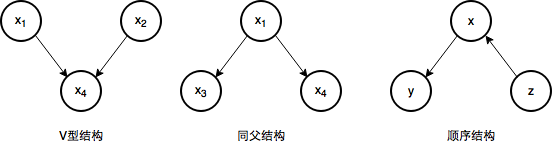
\includegraphics[scale=1, width=0.8\textwidth]{figure/BNrelation.png}
    \caption{贝叶斯网络中变量的典型依赖关系}
    \label{fig-bayes-dependence}
\end{figure}


在同父结构中,给定父节点$x_1$的值,则$x_3$和$x_4$条件独立,在顺序结构的依赖关系中,给定$x$的值,则$y$与$z$相互独立。在Y型结构中,如果说给定节点$x_4$的值,那么$x_1$$x_2$必然不独立。但是需要本文注意的是,如果说$x_4$的值未知,那么在V型结构下$x_1$$x_2$是互相独立的。这种独立性称为边际独立性(\textit{marginal Independence}),记作$x_1 \bot x_2$。

实际上,一个变量的取值的确定与否,能对另外两个变量之间的独立性发生影响,并非在这几个结构中特有的。一般来说,某个值确定与否,会对其他变量的独立性产生非常大的影响。

为了分析有向图中所有的V型之间的独立性,本文可以利用有向分离(D-Separation)。首先,本文将有向图转为一个无向图:

\begin{itemize}
	\item 找出有向图中所有的V型结构,在V型结构的两个父节点之间架上一条无向边;
	\item 将所有有向边改为无向边。
\end{itemize}

因此,由此产生的无向图称为道德图(moral graph),本文使得父节点相连的过程称为道德化(\textit{moralization})。

基于\textit{moral graph}本文能够非常直观地、迅速地找到变量之间的条件独立性,假定\textit{moral graph}中有变量$x, y$以及变量集合$\bm{z} = {z_i}$,如果变量$x$和$y$能够在图上被$z$分开,则从\textit{moral graph} 将变量集合$\bm{z}$除去之后,x和y分属两个连通分支,则称两者为有向分离,$x \bot y | \bm{z}$成立。



\subsection{马尔可夫随机场}

马尔科夫随机场(\textbf{Markov Random Field},简称MRF)是最经典的马尔科夫网络模型,是本文前面所说的无向图模型。模型图中每一个节点均表示相对应的某个变量,并且图中节点间的边表示节点所代表的两个变量的依赖关系。马尔科夫随机场模型中有称为势能函数(potential function),也称为因子(factor)函数,即为定义在变量集合上 main的非负实函数,用于定义所研究问题所需要的概率分布函数。

在马尔可夫随机场中,多个变量的联合概率分布能够基于场中的图团的分解为多个因子(factor)的乘积,即为每一个因子仅仅和一个团结构相关。具体来说,对于变量集合$\bm{X} = \{x_1, x_2, x_3..., x_n\}$,所有的团结构的结合为$C$,和团$Q \in C$对应的变量集合记为$\bm{x}_Q$,则所定义的联合概率$P(\bm{X})$定义为

\begin{equation}
	P(\bm{X}) = \frac{1}{Z} \prod_{Q \in C} \psi_Q(\bm{X}_Q) \\
	\label{eq-markov}
\end{equation}

\begin{equation}
Z = \sum_{\bm{x}} \prod_{Q \in C} \psi_Q(\bm{X}_Q) \\
\end{equation}


其中$\psi_Q$为和团$Q$一起对应的势能函数,用于对团$Q$中的各种变量的关系进行建模,\textit{Z}为规范化因子,以确保$P(\bm{X})$被正确定义的概率。在实际运用的时候,计算Z的值通常比较困难,但幸运的是,许多方法都可以通过近似计算来获取Z的取值。

显然易见,当网络中变量的数量越来越多的时候,则团里面的数目将会变得非常多(如两个相连的变量都会变成团结构),这就说明式\ref{eq-markov}会有非常多的乘积项,这显然会给模型带来非常多的计算量。并且,如果团结构$Q$不是极大团的话,则它一定会被一个极大团$Q^{\star}$所包含。既有$\bm{X}_Q \subseteq \bm{X}^{\star}$;这也说明变量$X_Q$之间的关系不仅仅在势能函数$\psi_Q$中进行了计算,也在势能函数$\psi_{Q^{\star}}$中进行了计算。由此本文可以将联合概率用极大团来重新进行定义。这里本文假设所有的极大团构成的集合为$C^{\star}$,则本文前面定义的联合概率可以重新改写为

\begin{equation}
	P(\bm{X}) = \frac{1}{Z^{\star}} \prod_{Q \in C^{\star}} \psi_Q(\bm{X}_Q) \\
\end{equation}


\begin{equation}
Z^{\star} = \sum_{\bm{x}} \prod_{Q \in C^{\star}} \psi_Q(\bm{X}_Q) \\
\end{equation}


这里的$Z^{\star}$为规范因子。


下面本文对马尔科夫随机场的独立性进行说明 \\
\begin{itemize}
\item 全局马尔科夫性(\textit{Global Markov Property}):给定两个变量集的分离集,则这两个变量集条件独立。 
\item 局部马尔科夫性(Local Markov property):给定某个变量的近邻变量,或者称为该变量的马尔科夫毯(Markov blanket),则该变量独立于其他的变量。用形式化语言来描述即为,让V为网络中的结点集合,$n(v)$为结点$v$在网络图中的近邻节点,$n^{\star}(v) = n(v)\cup \{v\}$,有$\bm{x}_v \perp \bm{x}_{V 	\backslash n^{\star}(v)} \mid \bm{x}_{n(v)} $ 

\item 成对的马尔科夫性(\textit{pairwise Markov property}):给定所有其他变量,两个非邻近变量条件独立。形式化语言来说,即令图中的节点集合和边的结合分别为$V$和$E$,对于网络图中的两个节点$u$和$v$,如果$<u,v> \notin E$,则$\bm{x}_u \perp \bm{x}_v \mid X_{V \backslash <u, v>}$。


\end{itemize}



除此之外,本文最后来对马尔科夫随机场的势能函数进行具体说明。很明显,势能函数$\psi_Q(\bm{x}_Q)$是定量的对变量集合$X_Q$中的变量之间的关系进行说明,即该函数应该为非负函数,并且在所喜好的变量取值有着较大的函数值。

而为了满足势能函数的非负性质,本文常常使用指数函数来定义势能函数,即为
\begin{equation}
\psi_Q(\bm{X}_Q) = \exp^{-H_Q(\bm{x}_Q)}
\end{equation}

$H_Q(\bm{x}_Q)$函数是一个定义在变量$\bm{x}_Q$上面的实数函数,常见的形势可以为
\begin{equation}
H_Q(\bm{x}_Q) = \sum_{u,v \in Q, u \neq v} \alpha_{uv} x_u x_v + \sum_{v \in Q} \beta_v x_v \\
\end{equation}

其中$\alpha_{uv}$、$\beta_v$为参数。 上面式子中第二项仅仅考虑单个节点,而第一项则考虑每对节点之间的关系。



\subsection{条件随机场}
条件随机场模型(Conditional Random Fields,简称CRF)\upcite{sutton2006introduction}是一种判别式的,且为无向图模型。前面第一张的研究中本文提到过生成式模型以及判别式模型。判别式模型为对条件概率分布进行建模,而生成式模型则是直接对联合概率分布进行建模。马尔科夫条件随机场以及贝叶斯网络均是生成式模型,而条件随机场为判别式模型。


与马尔科夫随机场不同的是,条件随机场试图在给定的观察值的条件下,对多个变量的条件概率进行建模。具体来说,让$x = \{x_1, x_2,...,x_n\}$为观察序列,$\bm{y} = \{y_1, y_2,...,y_n\}$为其与之对应的标记序列,那么条件随机场的目标首先即为构建基于条件概率分布的模型$P(\bm{y} \mid \bm{x})$。值得说明的是,这里的标记变量集合$\bm{y}$可以是结构性的变量,即有可能其分量之间本身就具有一定的相关性。例如在NLP领域当中的词类别标注任务当中,如果说可观测的变量为语句(即为单词序列),那么标记相应的词类别序列,即 $\bm{y}$具有线性结构。


下面本文对条件随机场模型进行定义。

让$G = <V,E>$ 表示图中的节点与标记变量$\bm{y}$中的元素对应的无向网络图。$y_i$表示与节点$i$对应的标记变量,$n(i)$表示节点
$i$的近邻节点集合,如果图$G$中每个节点都满足马尔科夫性质,即
\begin{equation}
P(y_i \mid \bm{x},\bm{y}_{V \backslash \{i\}}) = P(y_i \mid \bm{x}, \bm{y}_{n(i)}) \\
\end{equation}

则本文称$(\bm{y}, \bm{x})$构成一个条件随机场。


理论上来说,图$G$可以拥有任何结构,只需要它满足图中变量之间的条件独立性关系即可。但是,在现实世界应用中,特别是前面的标记序列建模的时候,最常用的仍然是本文前面所说到的链式结构,即链式条件随机场(chain-structured CRF)。下面本文仅仅对该形式的条件随机场进行具体分析,而任意图结构的条件随机场会在本文建模的时候得以体现,所以这里本文不进行介绍。



\begin{figure}[ht]
    \centering
    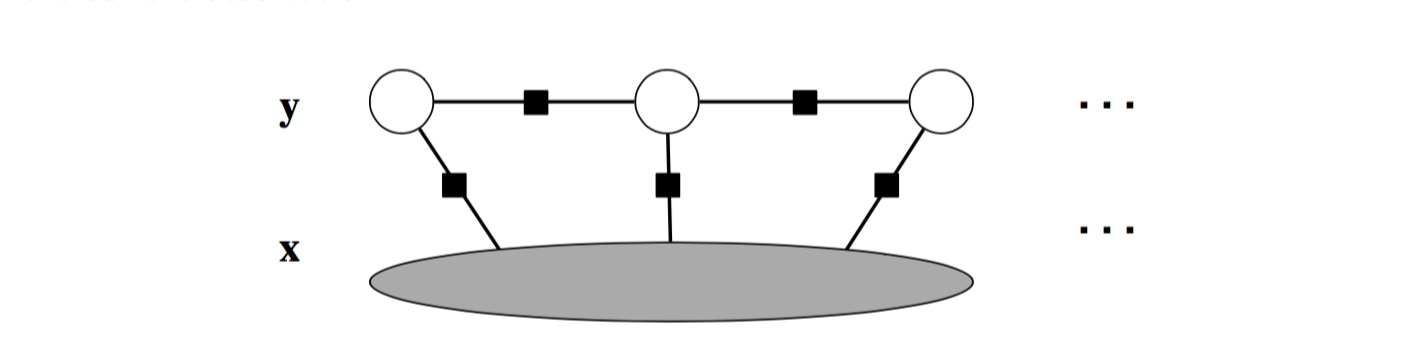
\includegraphics[scale=1, width=\textwidth]{figure/linearchain-crf.PNG}
    \caption{链式条件随机场模型实例}
    \label{fig-linear-crf}
\end{figure}


和本文前面介绍的马尔科夫随机场定义联合概率的方法相似,这里条件随机场定义使用势能函数以及图中的团结构来定义条件概率$P(\bm{y \mid x})$。在图\ref{fig-linear-crf}所显的链式条件随机场主要有两种已知标记变量的团结构,即单个标记变量$\{y_i\}$以及近邻的标记变量$\{y_{i-1}, y_i\}$。选择合适的势能函数,则可以得到如式\ref{eq-markov}的条件概率形式。在条件随机场里面,本文通过使用指数势能函数,并且引入特征函数的概念(feature function),条件概率即可以重新改写为
\begin{equation}
	P(\bm{y \mid x}) = \frac{1}{Z} \exp \bigg(\sum_j \sum_{i = 1}^{n - 1} \lambda_i t_j (y_{i+1}, y_j, \bm{x}, i) + \sum_{k} \sum_{i= 1}^{n} \mu_{k} s_{k}(y_i, \bm{x}, i) \bigg) \\
	\label{eq-lin-crf}
\end{equation}


其中$t_j (y_{i+1}, y_j, \bm{x}, i) $为定义在观察序列变量上面的邻近标记位置上的转移特征函数(transition feature function),这些函数常常用来描述相邻标记变量之间的定量关系以及观察序列对这些观察序列之间的影响。$s_{k}(y_i, \bm{x}, i) $为观察序列的标记位置i的状态特征函数(status feature function),这个是用来定量描述观察变量对于标记变量的影响。其中$\lambda_j$和$\mu_k$为待求解参数,Z为规范化因子,用于确保式子\ref{eq-lin-crf}的概率准确性。



对比\ref{eq-lin-crf}以及式\ref{eq-markov},本文可以知道,条件随机场以及马尔科夫随机场都用了团结构上面的势能函数来定义和求解概率,二者在形式上面并没有太大的区分,但是条件随机场使用的条件概率进行建模,而马尔科夫随机场使用的联合概率进行建模。



\subsection{网络中的学习与推断}
对于概率图模型中所定义的联合概率,本文能够用目标变量的边际分布(marginal distribution)或者用某些已知变量为条件来进行条件分布推断。在前面的介绍中本文已经知道了很多的条件概率建模,例如在隐式马尔可夫模型中估计观察序列在给定参数下的条件概率分布。这里的边际分布指的是对无关的变量进行求和或者进行积分之后而得到结果。例如,在马尔科夫网络中,网络中的变量的联合分布可以被表示成为极大团的势能函数的乘积,则在给定参数$\Theta$的条件下,求解某个变量$x$的分布,即成为了对于联合概率分布中其他的无关变量进行积分的过程,也被称为边际化(marginalization)。

对于概率图模型,求解的过程实质就是确定具体的未知参数分布,这也被称为参数估计或者参数学习问题。换个角度,如果将未知参数看作未知变量,那么参数估计的过程则和未知变量推断的过程非常相似。因此, 两个问题都可以归结为概率图模型中的推断问题。

概率图模型中的推断方法大致可以分为两大类\upcite{koller20072},第一类为精确推断,即通过数学推导的方法精确计算出目标变量的边际分布的准确值。但是,一般来说,此类方法的计算复杂度为指数级别,该类方法的使用范围有限。第二类则为近似推断的方法,即能够在较低的时间复杂度内实现对原来问题的近似求解。此类方法在现实研究中运用的更加常见,该类方法也主要分为两大类:即第一类为采样(sampling),采用随机采样的方法对结果进行近似求解;另外一类是变分推断(variational inference),即近似进行推断求解。在本文的问题中,本文为了算法效率的高效性,采用的是信念传播的近似求解,置信信念传播(Loopy Belief Propagation)进行参数的学习与推断。










